% !TEX root = ./../paper.tex

\section{Results}
\label{sec:results}

\subsection{Language Implementation}
\label{sec:results:language}

\sculpt as a programming language is a functioning language capable of writing any program.

The language uses FILO (First In Last Out) stacks as its only data structure to store and manipulate data. Each stack is represented by a different shape other than the reserved shapes used by the instructions, and they are initialized on first call.
Stacks can hold an arbitrarily large amount of rational numbers.
Stacks allow the pop, push, move and duplicate operations.
Numbers are defined by their literal counterparts, and the language supports basic arithmetic.
Regarding their representation, stacks are represented by any shape that is not reserved for the instructions,, such as simple shapes like circles, triangles or squares or complex drawings. Anything goes.

Arithmetic operations are the only operations available in \sculpt.
Available operations are addition, subtraction, multiplication, comparison, modulo and division.
These are performed in two ways:

\begin{itemize}
    \item \textbf{As unary operator}: The first two elements of the stack given by parameter are popped and operated and pushing the result back into the stack.
    \item \textbf{As binary operator}: The first element of the stack given by parameter is popped and the second parameter, a number, are operated with the result of the first operation. The result is pushed back into the stack.
\end{itemize}

In cases where the arithmetic is not defined, such as division by zero or modulo by zero, a \textit{nil} value is pushed into the stack.
When a \textit{nil} value is encountered on arithmetic operations, other than comparisons, the program will halt in an error state.

\sculpt allows for flow control through the use of loops, conditional blocks and jump blocks.
Loops are physically represented by a literal loop of connected blocks or a single block jump with a negative number as a parameter.
The jump block is a special block that allows for the execution to continue at any point by moving the execution from the current block to another with the offset given by parameter.
Conditional statements are represented by a question block using a stack value as a parameter. Positive values are considered true and evaluate the following block, and negative values are considered false and do not evaluate the affected block, but rather skips the next instruction.


\sculpt is based on the physical blocks. Blocks as three-dimensional objects are unwieldy to be described in text.
Therefore, we have made several valid notations for \sculpt programs.
Every block is represented as a square with the shape of each block inside the square.
The connections between blocks are represented by arrows between the squares.
As a first example and introduction to the language itself, we have implemented a simple program that calculates the Fibonacci sequence in \sculpt.

\begin{figure}[h]
    \centering
    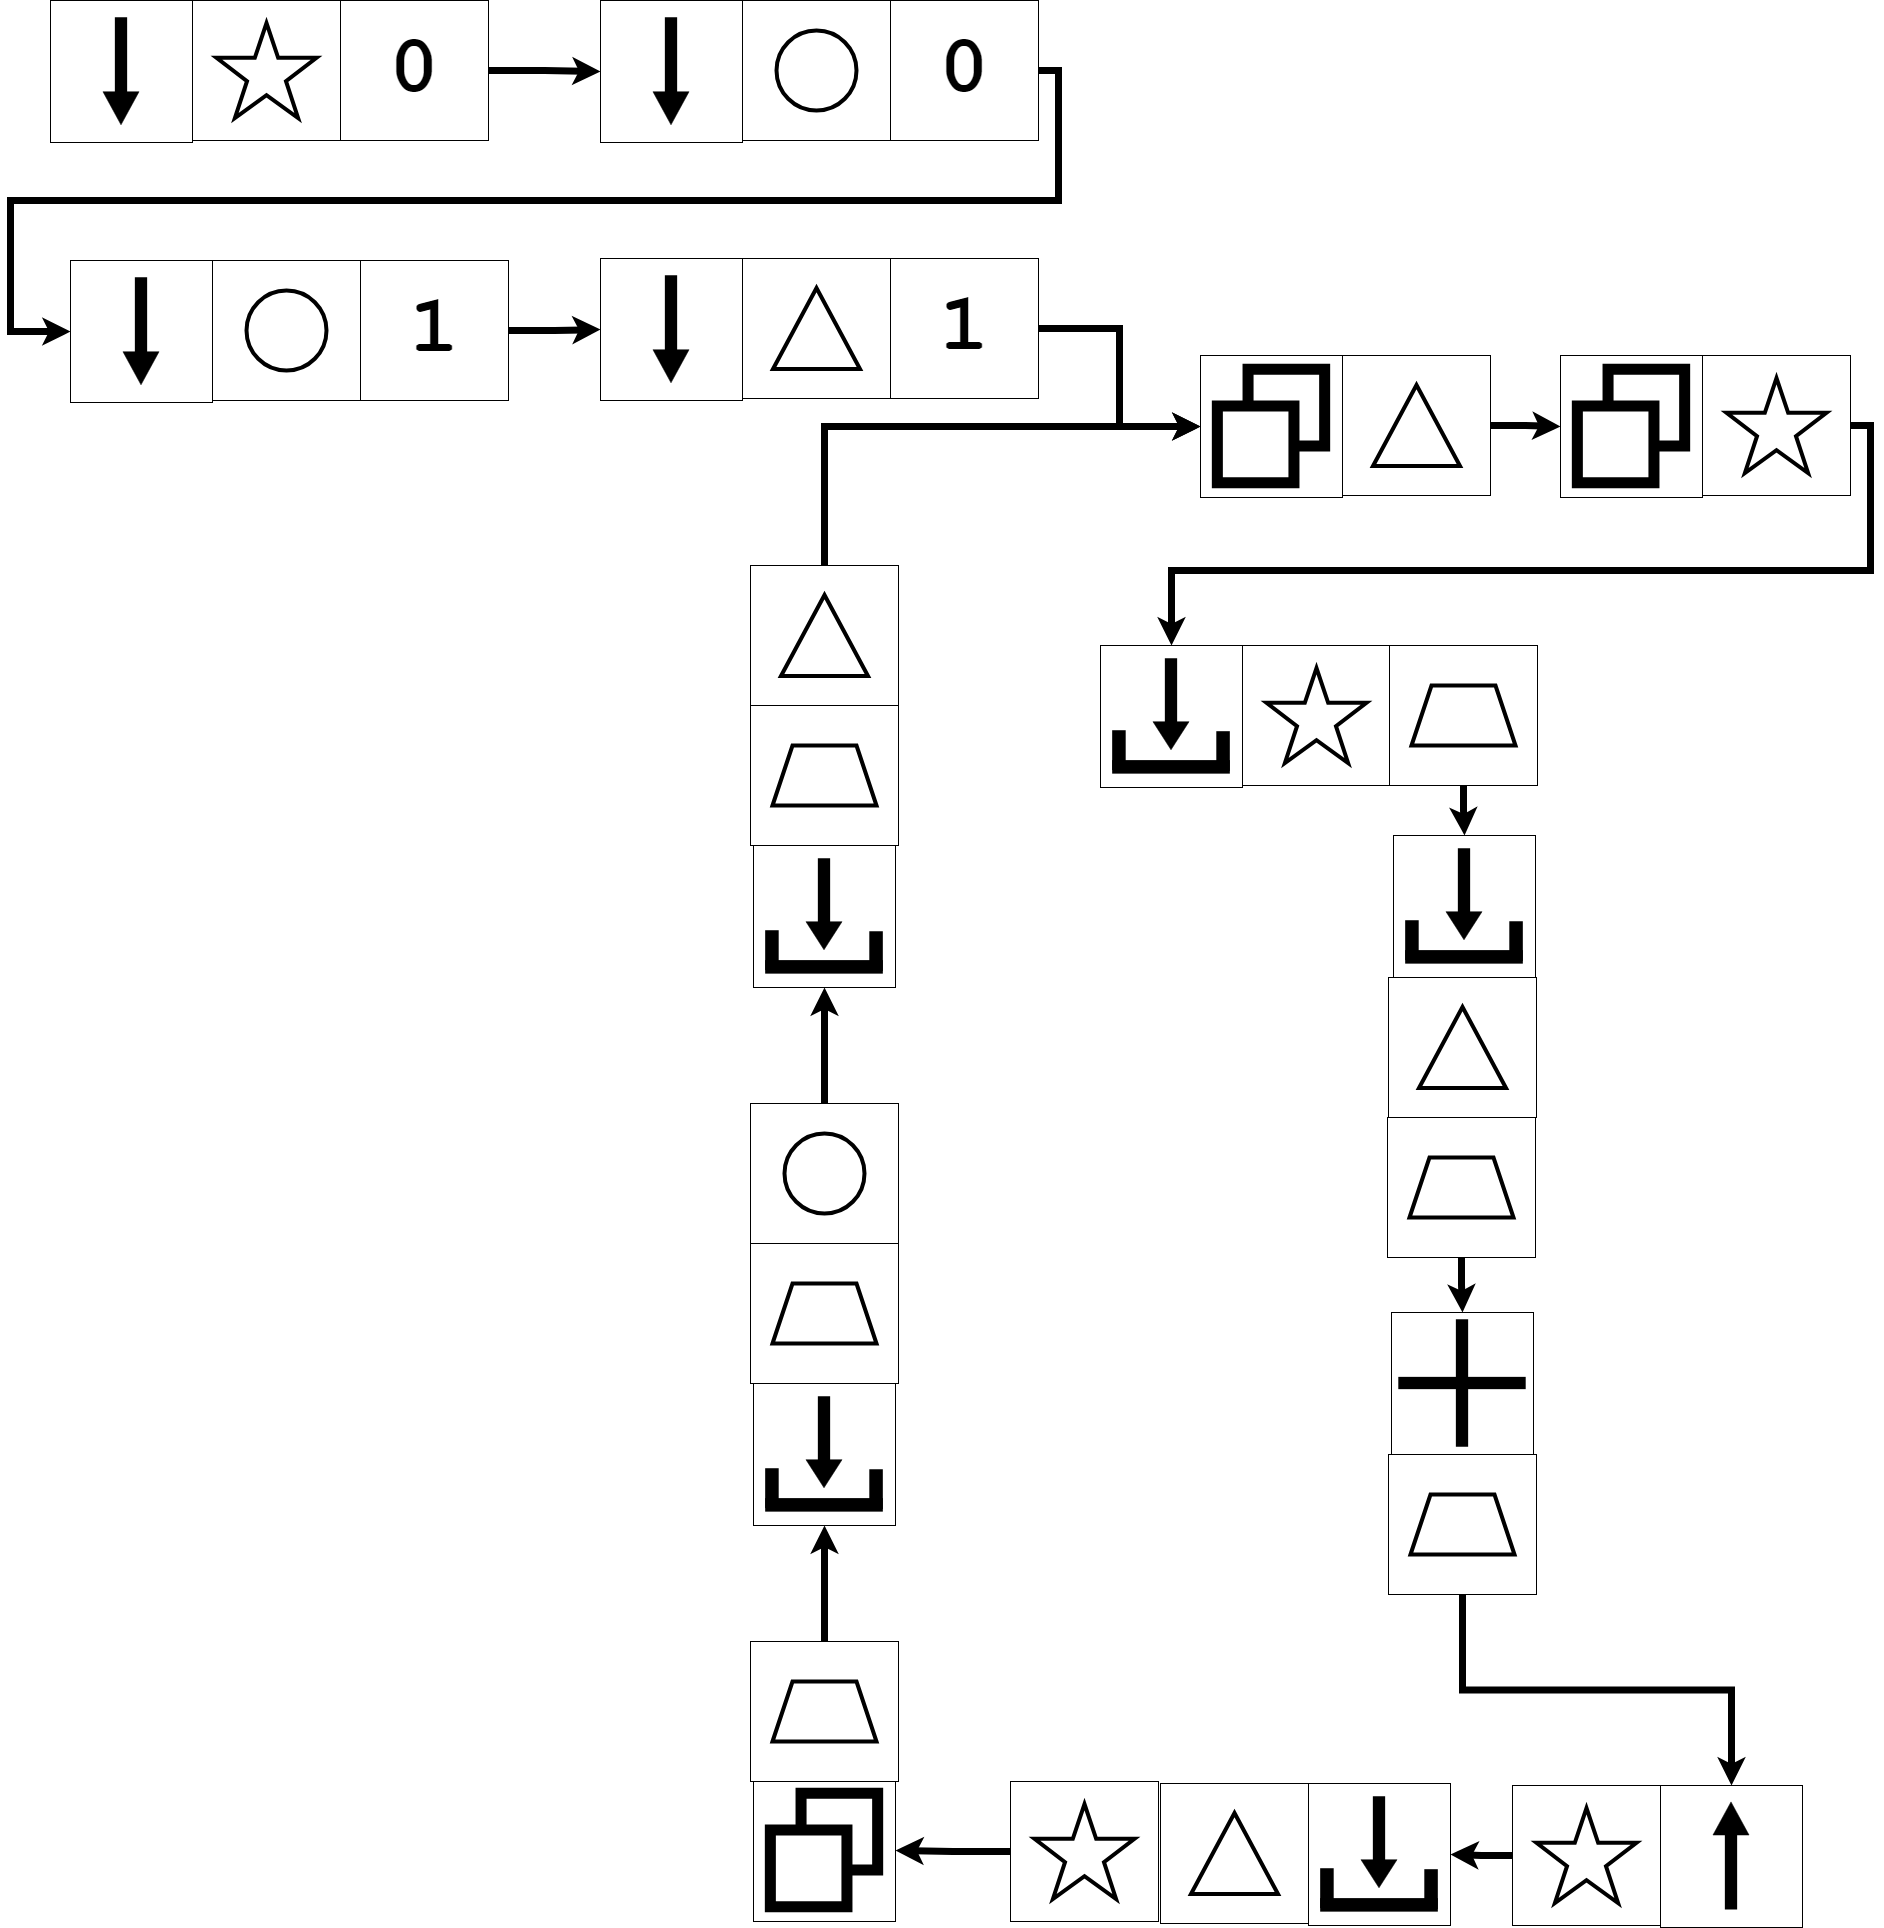
\includegraphics[width=0.5\textwidth]{figures/ArtlangFibpng}
    \caption{\sculpt Fibonacci program}
    \label{fig:artlangfib}
    \vspace{5pt}
\end{figure}

The program in Figure \ref{fig:artlangfib} fills the circle stack with the numbers of the Fibonacci sequence.

The second notation is a more traditional representation of code, which is used by the \sculpter interpreter, which will be explained afterwards.
The program is written in a more traditional way, every block has a reserved name, connections are omitted. It reads as a list of instructions, somewhat similar to an assembly language.
Limitations of this implementation are that the program is not visually represented, connections between blocks are not shown and physical loops cannot be represented, forcing the user to only use jump operations for execution control.
Our Fibonacci implementation can be rewritten in \sculpter as follows.

\begin{algorithm}
    \caption{Fibonacci sequence in \sculpt}
    \label{alg:fib}
    \small
    \begin{algorithmic}
    \State $push~0$ \textbf{star}
    \State $push~0$ \textbf{circle}
    \State $push~1$ \textbf{circle}
    \State $push~1$ \textbf{triangle}
    \State $dup$ \textbf{triangle}
    \State $dup$ \textbf{star}
    \State $mov$ \textbf{star} \textbf{trapezoid}
    \State $mov$ \textbf{triangle} \textbf{trapezoid}
    \State $add$ \textbf{trapezoid}
    \State $pop$ \textbf{star}
    \State $mov$ \textbf{triangle} \textbf{star}
    \State $dup$ \textbf{trapezoid}
    \State $mov$ \textbf{trapezoid} \textbf{circle}
    \State $mov$ \textbf{trapezoid} \textbf{triangle}
    \State $jmp$ \textbf{-10}
    \end{algorithmic}
    \end{algorithm}


Writing a Fibonacci program is a simple task in \sculpt which gives us a good insight on how \sculpt looks and feels, yet it is not a complete proof of the language's capabilities.
The language is Turing complete and it is capable of writing any program that can be written in any other programming language.
To validate this, we will simulate a Turing machine in \sculpt.
For this instance, an implementation of a 3-State Busy Beaver Turing machine will be used.

Its \sculpter implementation is as follows:

\begin{algorithm}[H]
    \caption{3-State Busy Beaver Turing machine in \sculpt}
    \label{alg:busybeaver}
    \small
    \begin{algorithmic}
    \State $push~0$ \textbf{left}
    \State $push~0$ \textbf{left}
    \State $push~0$ \textbf{left}
    \State $push~0$ \textbf{left}
    \State $push~0$ \textbf{right}
    \State $push~0$ \textbf{right}
    \State $push~0$ \textbf{right}
    \State $push~0$ \textbf{right}
    \State $push~0$ \textbf{head}
    \State \textbf{// STATE A}
    \State $push~1$ \textbf{temp}
    \State $mov$ \textbf{temp} \textbf{head}
    \State $cmp$ \textbf{temp}
    \State $?$ \textbf{temp}
    \State $jmp~13$ \textbf{// Go to A\_1}
    \State $push~1$ \textbf{head}
    \State $mov$ \textbf{right} \textbf{head}
    \State $mov$ \textbf{head} \textbf{left}
    \State \textbf{// STATE B}
    \State $push~1$ \textbf{temp}
    \State $mov$ \textbf{temp} \textbf{head}
    \State $cmp$ \textbf{temp}
    \State $?$ \textbf{temp}
    \State $jmp~9$ \textbf{// Go to B\_1}
    \State $push~1$ \textbf{head}
    \State $mov$ \textbf{left} \textbf{head}
    \State $mov$ \textbf{head} \textbf{right}
    \State $jmp~-16$ 
    \State \textbf{// A\_1}
    \State $push~1$ \textbf{head}
    \State $mov$ \textbf{left} \textbf{head}
    \State $mov$ \textbf{head} \textbf{right}
    \State $jmp~5$ \textbf{// Go to C}
    \end{algorithmic}
\end{algorithm}

\begin{algorithm}[H]
    \caption{3-State Busy Beaver Turing machine in \sculpt (continued)}
    \label{alg:busybeaver}
    \small
    \begin{algorithmic}
    \State \textbf{// B\_1}
    \State $push~1$ \textbf{head}
    \State $mov$ \textbf{right} \textbf{head}
    \State $mov$ \textbf{head} \textbf{left}
    \State $jmp~-16$ \textbf{// Go to B}
    \State \textbf{// STATE\_C}
    \State $push~1$ \textbf{temp}
    \State $mov$ \textbf{temp} \textbf{head}
    \State $cmp$ \textbf{temp}
    \State $?$ \textbf{temp}
    \State $jmp~5$ \textbf{// Go to HALT}
    \State $push~1$ \textbf{head}
    \State $mov$ \textbf{left} \textbf{head}
    \State $mov$ \textbf{head} \textbf{right}
    \State $jmp~-25$ \textbf{// Go to B}
    \State \textbf{// HALT}
    \State $push~1$ \textbf{head}
    \end{algorithmic}
\end{algorithm}

\normalsize
This simulation of the Busy Beaver Turing machine is a simple program that runs for some time before halting.
Since this simulation is of a Turing machine, it is capable of simulating any algorithm, thus proving that \sculpt is Turing complete.

The complete implementation of \sculpt is open source and is available on GitHub\footnote{\url{https://github.com/Darkoyd/SCuLPT}}.

\subsection{Interpreter Implementation}
\label{sec:results:interpreter}
\sculpter is an interpreter for \sculpt built in Scala that allows users to write and execute \sculpt programs in a more traditional way.
It leverages the Scala.js framework to provide a web-based interface for users.
This makes the interpreter lightweight, distributable and easy to use without the need for any additional software.
\sculpter features a simple text editor where a program can be written. It also features buttons to lex, parse and execute the program.
Execution of the program is done in a step-by-step manner, allowing users to see the state of the program at each step.
\sculpter code is open source and is also available on GitHub\footnote{\url{https://github.com/Darkoyd/SCuLPTER}}.


\subsection{Validation}
\label{sec:results:validation}
To validate \sculpt, we have conducted a series of sessions with different users to test the language and its ecosystem.
A total of 6 sessions were conducted with a total of 75 users, ranging from novices with no prior programming experience to expert programmers with years of experience in the field.
The sessions were designed to evaluate the usability and accessibility of \sculpt, as well as the overall user experience of using the language.

\subsubsection{Regarding Usability}
\label{sec:results:validation:usability}
Usability was evaluated through questions in the survey given to users after the sessions, as well as through user interviews.
The results of the usability questionnaire showed that users found \sculpt, from a physical standpoint, to be easy to use and understand, 
with a majority of users reporting that they were able to use and understand the shapes and blocks of the language with relative ease.
Among the users, especially the younger demographics, the physicality of the blocks was a key factor in their understanding of the language.

One concern that was raised by the researchers was that of overall piece integrity and the possibility of losing pieces.
Continuous use of the blocks in a classroom setting could lead to pieces being lost or damaged, which could hinder the usability of the language.
PLA is a material notorious for being a somewhat soft plastic prone to deformation and damage, especially with repeated use.
As expected, some pieces were lost during the sessions, but the overall integrity of the blocks was maintained.
The blocks were able to withstand the repeated use and manipulation by the users. The remaining pieces were still usable and intact, and the users were able to continue using the language without any issues.

These results shows that \sculpt as a building block construct and visual language performs as expected, with users sharing overall positive feedback regarding the usability of the language.

\subsubsection{Regarding Computation}
\label{sec:results:validation:computation}

Another section of the survey was dedicated to evaluate, from a more technical eye, the ease of use of \sculpt as a programming language.
Alongside the survey, users were given a set of programming tasks to complete using \sculpt.
The tasks were designed to test the users' understanding of the language and its capabilities, as well as their ability to write programs in \sculpt.
Throughout the sessions, about 50\% of the total participants were able to complete the tasks.
Further, per-session analysis shows interesting insights into the users' understanding of the language.
The first session was conducted with a group of novice teenage users, who had no prior programming experience.
These users were able to understand the basic concepts of \sculpt yet they were not able to complete the tasks.
The second session was conducted with a group of undergraduate students and expert programmers, who had years of experience in the field.
Surprisingly, these users were also not able to complete the tasks, but they were able to understand the language and its capabilities.
The next sessions were conducted with groups ranging from children to teenagers. Children evidently struggled with programming, yet outshines in the physical manipulation of the blocks.
Teenagers, on the other hand, were able to understand the language and its capabilities, and they were able to complete the tasks in an average time of 1 hour and a half.

Results show that \sculpt as a programming language can be easy to understand and use, yet it is not easy to write programs in \sculpt.
The language is capable of writing any program, but it requires a certain level of understanding of the language and its capabilities.
This is a common issue with programming languages that \sculpt tried to eliminate, but it is still present.

\subsubsection{Regarding Aesthetics}
\label{sec:results:validation:aesthetics}
Special sessions were held with a group of artists to test their overall experience with \sculpt from their experience as artists.
Results were surprisingly positive, with most users reporting that they enjoyed very much the experience of using \sculpt.
Participants expressed their appreciation for the physicality of the blocks and the ability to manipulate them in a tangible way.
The physicality of the block "was quintessential to their experience".
Participants also reported that the blocks were easy to understand and use, and that they enjoyed the process of building their sculptures.
When presented with the programming tasks, participants were able to easily understand the assignments, understand the block and their functionalities, but they were not able to complete any task.
Nevertheless, they expressed overall satisfaction while trying and failing to complete the tasks.
Participants reported that the experience of using \sculpt was enjoyable and that they would like to use it again in the future.
This last point lead to additional sessions with the same group of artists, as they were engaged with \sculpt and wanted to explore it further.
While trying and failing to complete the tasks, they used the blocks to create sculptures that were not intended to be functional, but rather artistic.
Participants reported that they enjoyed the process of creating sculptures and that they found it to be a rewarding experience.
Surprisingly, participants used the blocks in ways that were not intended from the start. Creating visually interesting constructs with this newfound freedom.

These results paint \sculpt as a visually interesting, and even fun, medium for creative expression.
Although this document has been focused on \sculpt from a technical standpoint, it is important to note that \sculpt was not only made to be a programming language, but also a medium for creative expression.
\endinput